% --- SLIDES : Challenge 2 ---

\section{Challenge 2 : Vote for Pedro}

\begin{frame}{Objectifs du challenge}
\centering
{\LARGE Forger une signature RSA valide}\\
\begin{figure}
    \centering
    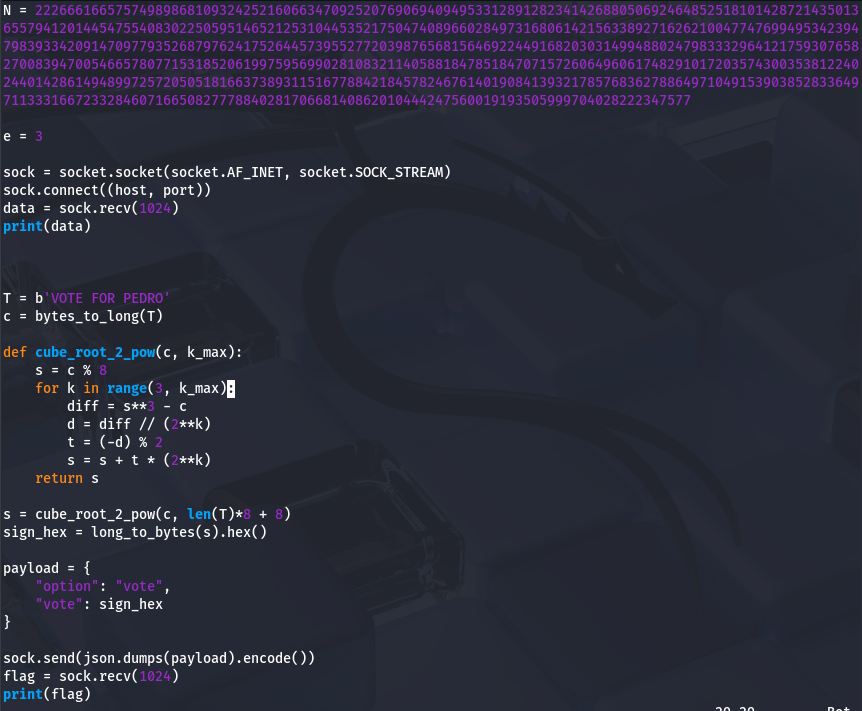
\includegraphics[width=0.5\textwidth]{scriptCh2.png}
\end{figure}
\vspace{0.1cm}
\begin{itemize}
    \item Voter pour Pedro sans clé privée
    \item Exploiter l'exposant faible $e = 3$
    \item Obtenir le flag
\end{itemize}
\end{frame}

\begin{frame}{Méthode de résolution}
\centering
{\LARGE Attaque par racine cubique}
\vspace{0.5cm}
\begin{align*}
\text{Signature } s &= \sqrt[3]{\text{Message}} \\
s^3 &\equiv \text{Message} \pmod{N}
\end{align*}
\begin{itemize}
    \item Message court = "VOTE FOR PEDRO"
    \item Pas de padding = vulnérabilité
\end{itemize}
\end{frame}


\begin{frame}{Résultat et Flag}
\centering
{\LARGE Signature forgée validée !}
\begin{figure}
    \centering
    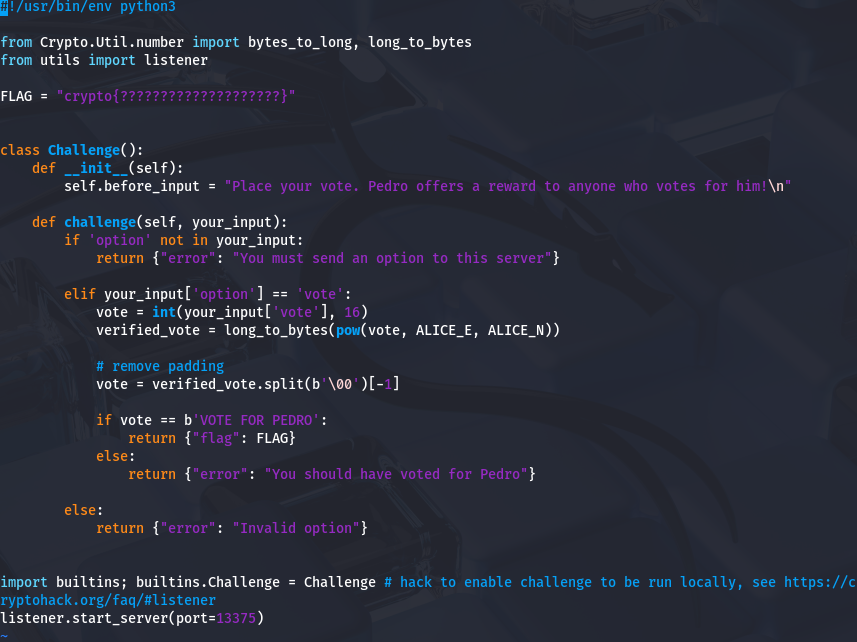
\includegraphics[width=0.5\textwidth]{scriptInitCh2.png}
\end{figure}
\vspace{0.1cm}
\begin{block}{Flag obtenu}
\texttt{crypto\{y0ur\_v0t3\_i5\_my\_v0t3\}}
\end{block}
\begin{itemize}
    \item Vote accepté par le serveur
\end{itemize}
\end{frame}